% Figure 5.4: NCF (Neural Collaborative Filtering) Architecture
% Compile with: pdflatex fig_5_4_ncf_architecture.tex

\documentclass[border=10pt]{standalone}
\usepackage{tikz}
\usetikzlibrary{shapes.geometric, arrows.meta, positioning, decorations.pathreplacing}
\usepackage{xcolor}

% Professional academic color palette
\definecolor{inputgray}{RGB}{220, 220, 220}
\definecolor{embedblue}{RGB}{176, 196, 222}    % Light steel blue
\definecolor{branchorange}{RGB}{222, 184, 135} % Burlywood
\definecolor{fusiongreen}{RGB}{176, 208, 176}  % Sage green
\definecolor{outputpurple}{RGB}{186, 175, 201} % Lavender gray
\definecolor{textdark}{RGB}{33, 33, 33}
\definecolor{accentblue}{RGB}{70, 130, 180}    % Steel blue

\begin{document}
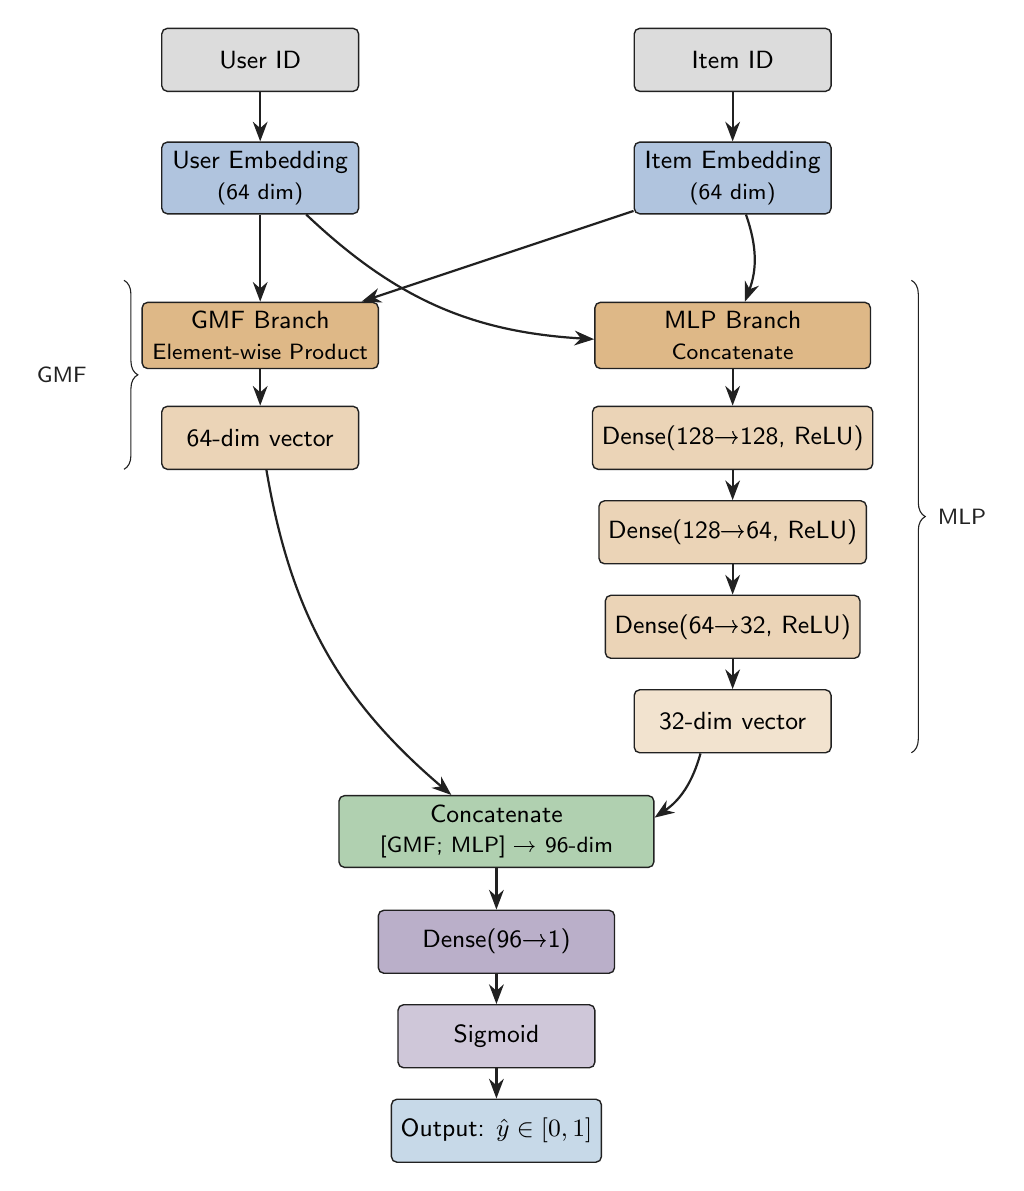
\begin{tikzpicture}[
    node distance=1cm,
    layer/.style={rectangle, draw=textdark, rounded corners=2pt, minimum width=2.5cm, minimum height=0.8cm, align=center, font=\small\sffamily, line width=0.5pt},
    embed/.style={layer, fill=embedblue},
    branch/.style={layer, fill=branchorange},
    fusion/.style={layer, fill=fusiongreen},
    output/.style={layer, fill=outputpurple},
    arrow/.style={-{Stealth[length=2.5mm]}, thick, color=textdark},
    brace/.style={decorate, decoration={brace, amplitude=5pt, raise=2pt}}
]

% Input
\node[layer, fill=inputgray] (userid) at (-3, 6) {User ID};
\node[layer, fill=inputgray] (itemid) at (3, 6) {Item ID};

% Embeddings
\node[embed] (useremb) at (-3, 4.5) {User Embedding\\{\footnotesize\sffamily (64 dim)}};
\node[embed] (itememb) at (3, 4.5) {Item Embedding\\{\footnotesize\sffamily (64 dim)}};

\draw[arrow] (userid) -- (useremb);
\draw[arrow] (itemid) -- (itememb);

% GMF Branch
\node[branch, minimum width=3cm] (gmf) at (-3, 2.5) {GMF Branch\\{\footnotesize\sffamily Element-wise Product}};
\node[layer, fill=branchorange!60] (gmfout) at (-3, 1.2) {64-dim vector};

% MLP Branch
\node[branch, minimum width=3.5cm] (mlp) at (3, 2.5) {MLP Branch\\{\footnotesize\sffamily Concatenate}};
\node[layer, fill=branchorange!60] (mlp1) at (3, 1.2) {Dense(128→128, ReLU)};
\node[layer, fill=branchorange!60] (mlp2) at (3, 0) {Dense(128→64, ReLU)};
\node[layer, fill=branchorange!60] (mlp3) at (3, -1.2) {Dense(64→32, ReLU)};
\node[layer, fill=branchorange!40] (mlpout) at (3, -2.4) {32-dim vector};

% Arrows for embeddings to branches
\draw[arrow] (useremb) -- (gmf);
\draw[arrow] (itememb) -- (gmf);
\draw[arrow] (useremb) to[bend right=20] (mlp);
\draw[arrow] (itememb) to[bend left=20] (mlp);

% GMF path
\draw[arrow] (gmf) -- (gmfout);

% MLP path
\draw[arrow] (mlp) -- (mlp1);
\draw[arrow] (mlp1) -- (mlp2);
\draw[arrow] (mlp2) -- (mlp3);
\draw[arrow] (mlp3) -- (mlpout);

% Fusion
\node[fusion, minimum width=4cm] (concat) at (0, -3.8) {Concatenate\\{\footnotesize\sffamily [GMF; MLP] → 96-dim}};
\draw[arrow] (gmfout) to[bend right=20] (concat);
\draw[arrow] (mlpout) to[bend left=20] (concat);

% Output
\node[output, minimum width=3cm] (dense) at (0, -5.2) {Dense(96→1)};
\node[output, fill=outputpurple!70] (sigmoid) at (0, -6.4) {Sigmoid};
\node[layer, fill=accentblue!30] (out) at (0, -7.6) {Output: $\hat{y} \in [0,1]$};

\draw[arrow] (concat) -- (dense);
\draw[arrow] (dense) -- (sigmoid);
\draw[arrow] (sigmoid) -- (out);

% Annotations
\draw[brace, color=textdark] (-4.8, 3.2) -- (-4.8, 0.8) node[midway, left=8pt, font=\footnotesize\sffamily] {GMF};
\draw[brace, color=textdark] (5.2, 3.2) -- (5.2, -2.8) node[midway, right=8pt, font=\footnotesize\sffamily] {MLP};

\end{tikzpicture}
\end{document}
